\chapter{Temporal Analysis of the Design and Development of Mobile Applications}
\label{ch:findings_chapter}
The trends in designing and developing mobile applications are always changing and evolving over time.
Platform owners regularly introduce new features, remove previous ones, and change their best practices and guidelines.
Since all of these changes are observed at some points in time, it is necessary to apply a temporal (time series) based analysis to capture interesting events and draw more meaningful statistical insights.
Temporal analysis enables us to ask new questions and understand the changes in the design and development of mobile applications.
The lack of effective retrieval systems and resources that provide access to the temporal nature of applications have limited the questions we might ask and resulted in studies that focus on a single snapshot in time.
Sieveable is what gives us access to the temporal nature of mobile applications and helps us to answer diverse analysis questions.
In this chapter, I present some illustrative temporal analysis examples to understand how apps are evolved over time in three areas: UI design, accessibility, and privacy.\footnote{The raw data, source code, and a set of interactive data visualizations are available at https://github.com/sieveable/sieveable-mining}.

\section{Visual Design Mining}

Mobile UI design guidelines are constantly updated to provide a better and consistent user experience across the platform.
For instance, in June 2014, Google introduced material design, a design specification language that makes use of elements from print design, responsive transitions, and depth effects \cite{Google_Material_Design}.
Since the concepts were announced, several third-party implementations have been built and used by developers.
A year after the announcement, Google introduced an official library called the Android Design Support Library, which allows developers to implement a number of material design components that are backward compatible with old devices.
Now, it has been over two years of efforts invested in creating concepts and tools to promote the use of this design language.
We can use Sieveable to understand how these concepts are adopted over time and ask questions like:
What is the state of adopting material design patterns?
Did these concepts get adopted immediately by developers or at slow pace?
Are there any factors that may have contributed into a sudden increase or decrease in adoption?

\subsection{Material Design Components}
In this section, I present a set of analyses on the adoption rate of two major material design components: the floating action button and the navigation drawer.
The floating action button is arguably the most recognizable material design component and  represents the primary action in an app.
The navigation drawer is perhaps the first design pattern that was introduced before material design and later was added to the design language.

\subsubsection{Floating Action Button}
\begin{figure}[H]
	\centering
	{{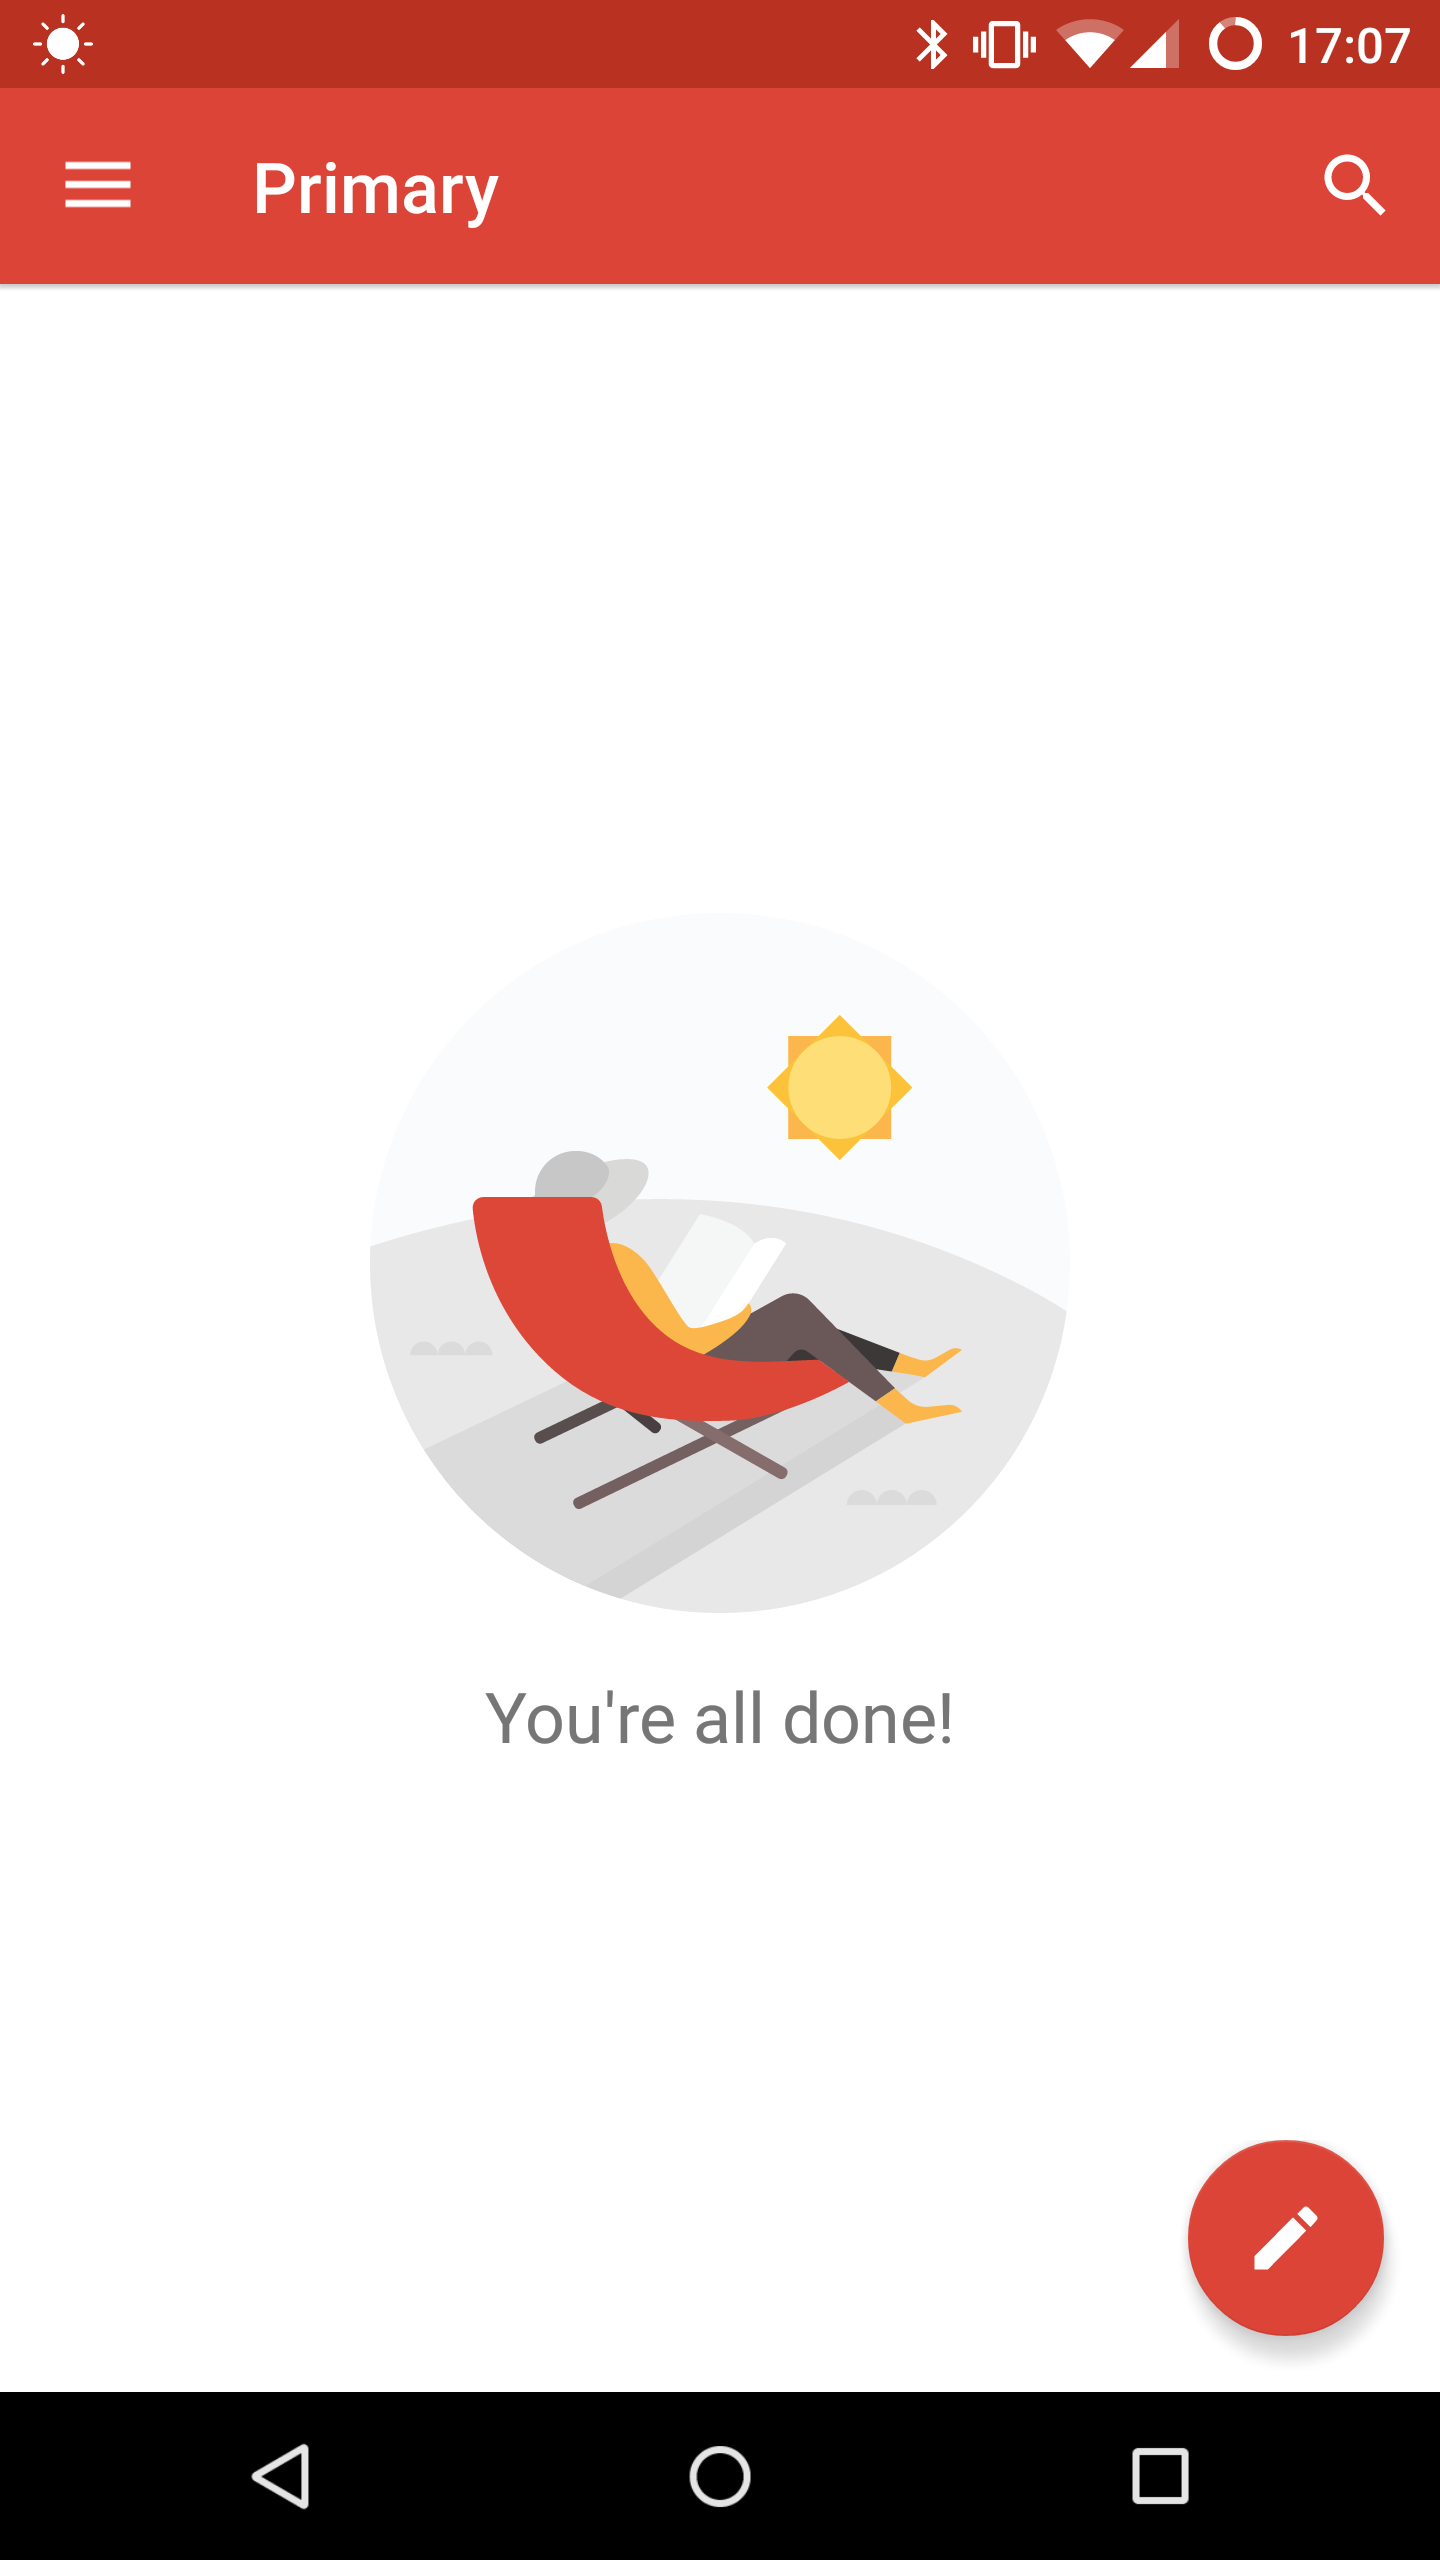
\includegraphics[scale=0.1]{figures/findings/fab-Gmail.png} }}%
	\qquad
	{{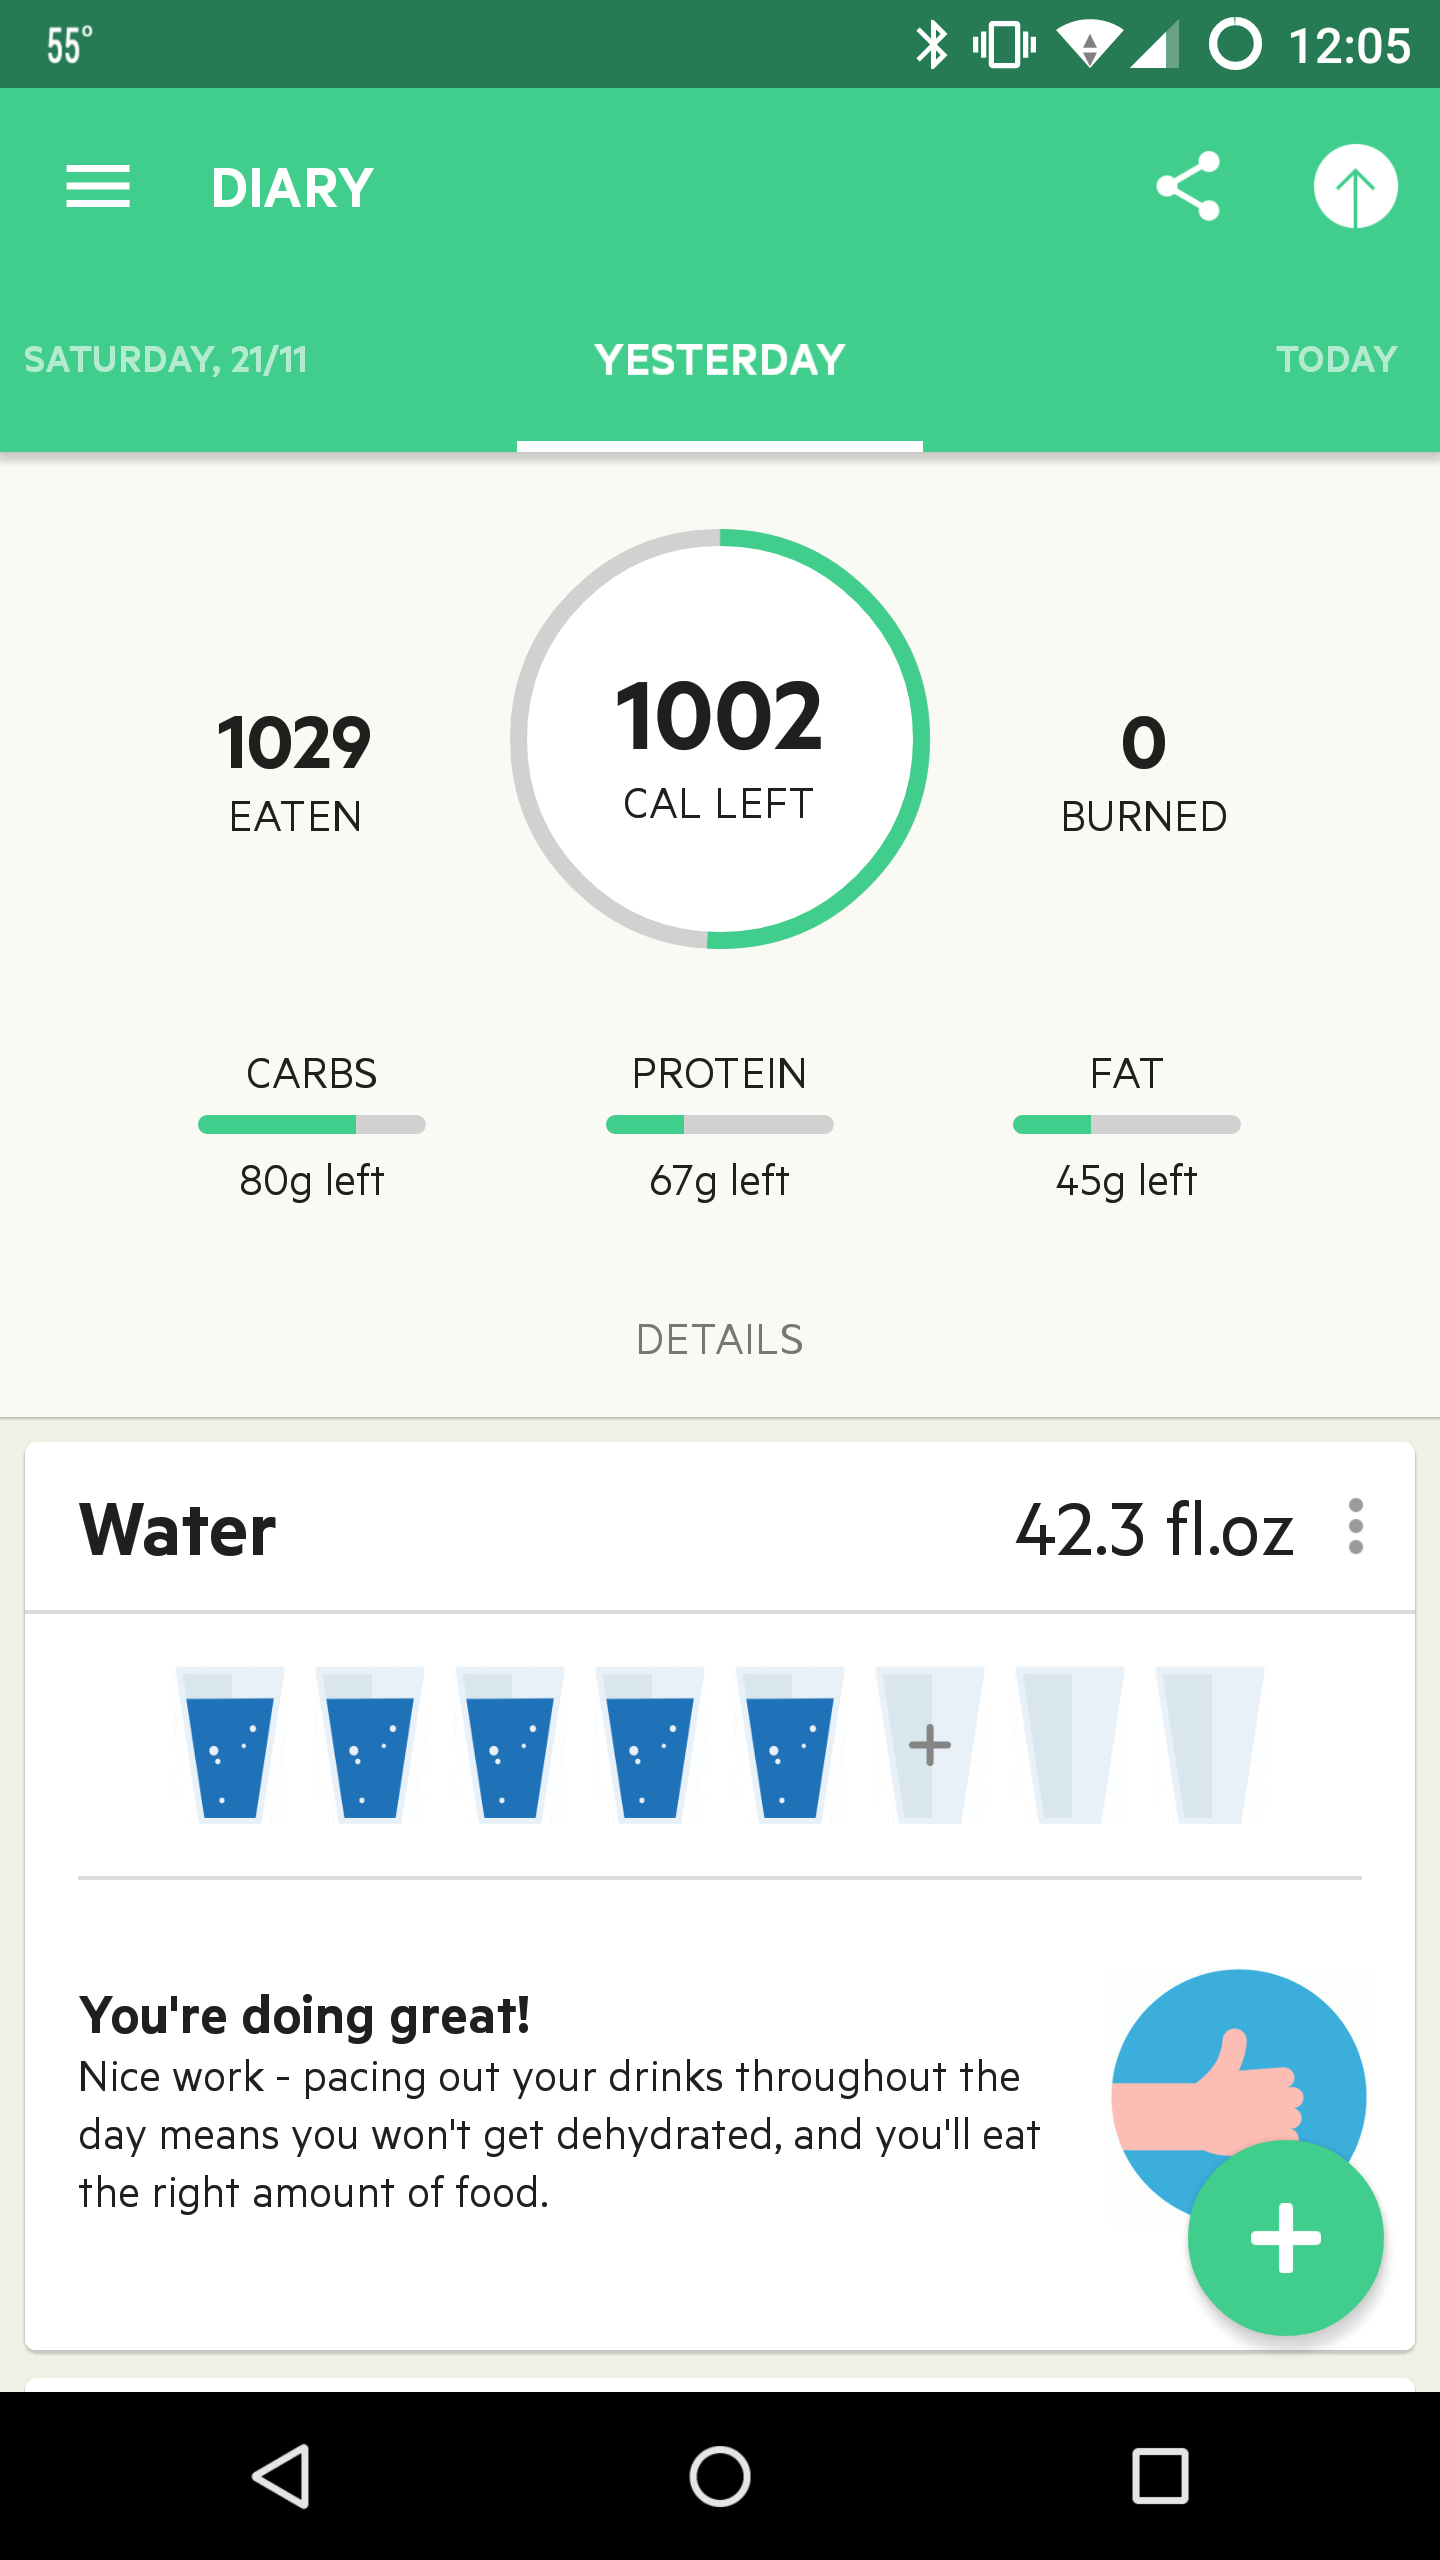
\includegraphics[scale=0.1]{figures/findings/fab-lifesum.png} }}%
	\caption{The Floating Action Button (FAB) shown at the bottom right corner of two apps, Gmail and Lifesum}%
	\label{fig:figure_fab_screenshot}
\end{figure}
The Floating Action Button (FAB) is a circled button floating above the UI to promote the primary action in the app (Figure~\ref{fig:figure_fab_screenshot}).
While developers can create a custom FAB with material design style, there are a few libraries that simplify adding this widget.
To find apps that have this UI component, one will write custom scripts to parse large number of UI layout files and count for all possible implementation options.
This task is achieved by writing a simple search query in Sieveable.
We can use Sieveable to evaluate implementation alternatives and help developers make an informed decision of using a specific library over others.
With Sieveable, one can examine the popularity of a specific UI library within any time window.
This can also provide insightful feedback to UI framework engineers on how well their efforts are received by developers.
We can find the trends of adopting the FAB as a design pattern over time using different alternatives.
At the time of writing, there are four common alternative ways to implement the FAB in Android: the official design support library \cite{Android_Design_Support_Lib}, and three other additional third-party libraries \cite{android-floating-action-button, FloatingActionButton, fab}.
I use the following Sieveable search queries to retrieve a set of apps that implement the FAB using the previously mentioned libraries: 

\inputminted
[
framesep=2mm,
baselinestretch=1.2,
bgcolor=MyLightGrayColor,
fontsize=\footnotesize
]
{xml}{figures/source-code/fab.txt}

\noindent When we combine all the results together and aggregate by the release year in which the first adoption is observed, we can get a sense of the adoption rate of the FAB over the last years as shown in figure~\ref{fig:fab_years}.
\begin{figure}[h]
	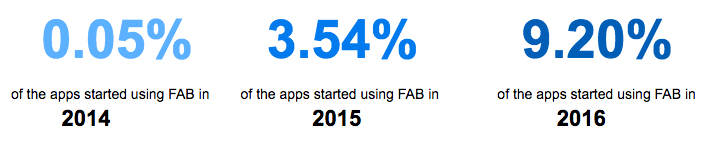
\includegraphics[scale=0.6]{figures/findings/fab_over_years.png}
	\caption{The adoption rate of the Floating Action Button (FAB) over the years.}
	\label{fig:fab_years}
\end{figure}
This shows that the adoption rate of this design pattern is growing slowly since it was first introduced in June 2014.
We can also analyze the adoption rate of the different implementation or library options over time.
\begin{figure}[h]
	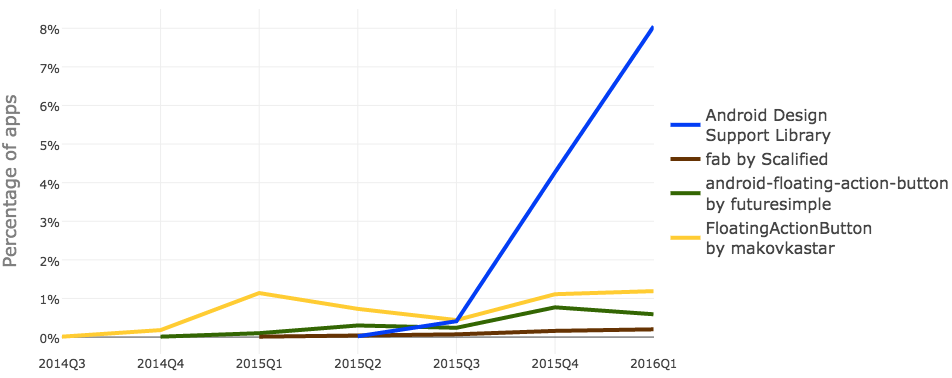
\includegraphics[scale=0.5]{figures/findings/fab_by_quarter.png}
		\caption{The percentage of apps that started adopting the Floating Action Button (FAB) using four popular libraries by calendar quarter.}
	\label{fig:fab_by_quartert}
\end{figure}
In Figure~\ref{fig:fab_by_quartert}, we can see that apps started adopted this pattern before the official release.
Once the official library was introduced by Google in May 2015 \cite{android_design_support_lib_blog_post}, the adoption rate started to increase noticeably.
This shows that a small number developers tend to use third-party libraries to implement a new design that is not yet officially supported.
The larger number of developers, however, are much quicker to use a consistent implementation by an official library.
Finally, I analyzed the group of apps that started adding FAB earlier using a third-party library before the existence of the official library.
I found that the majority of these apps have a low number of downloads (89.81\% with 100,000 download times or less compared to 10.19\% with more than 100,000 download times).
%\todo[inline]{TODO: How big is FAB apps with respect to all material design apps?}

\subsubsection{Navigation Drawer}
\begin{figure}[H]
	\centering
	{{
\includegraphics[scale=0.1]{figures/findings/closed-nav-drawer-kitchenstories.png} }}%
	\qquad
	{{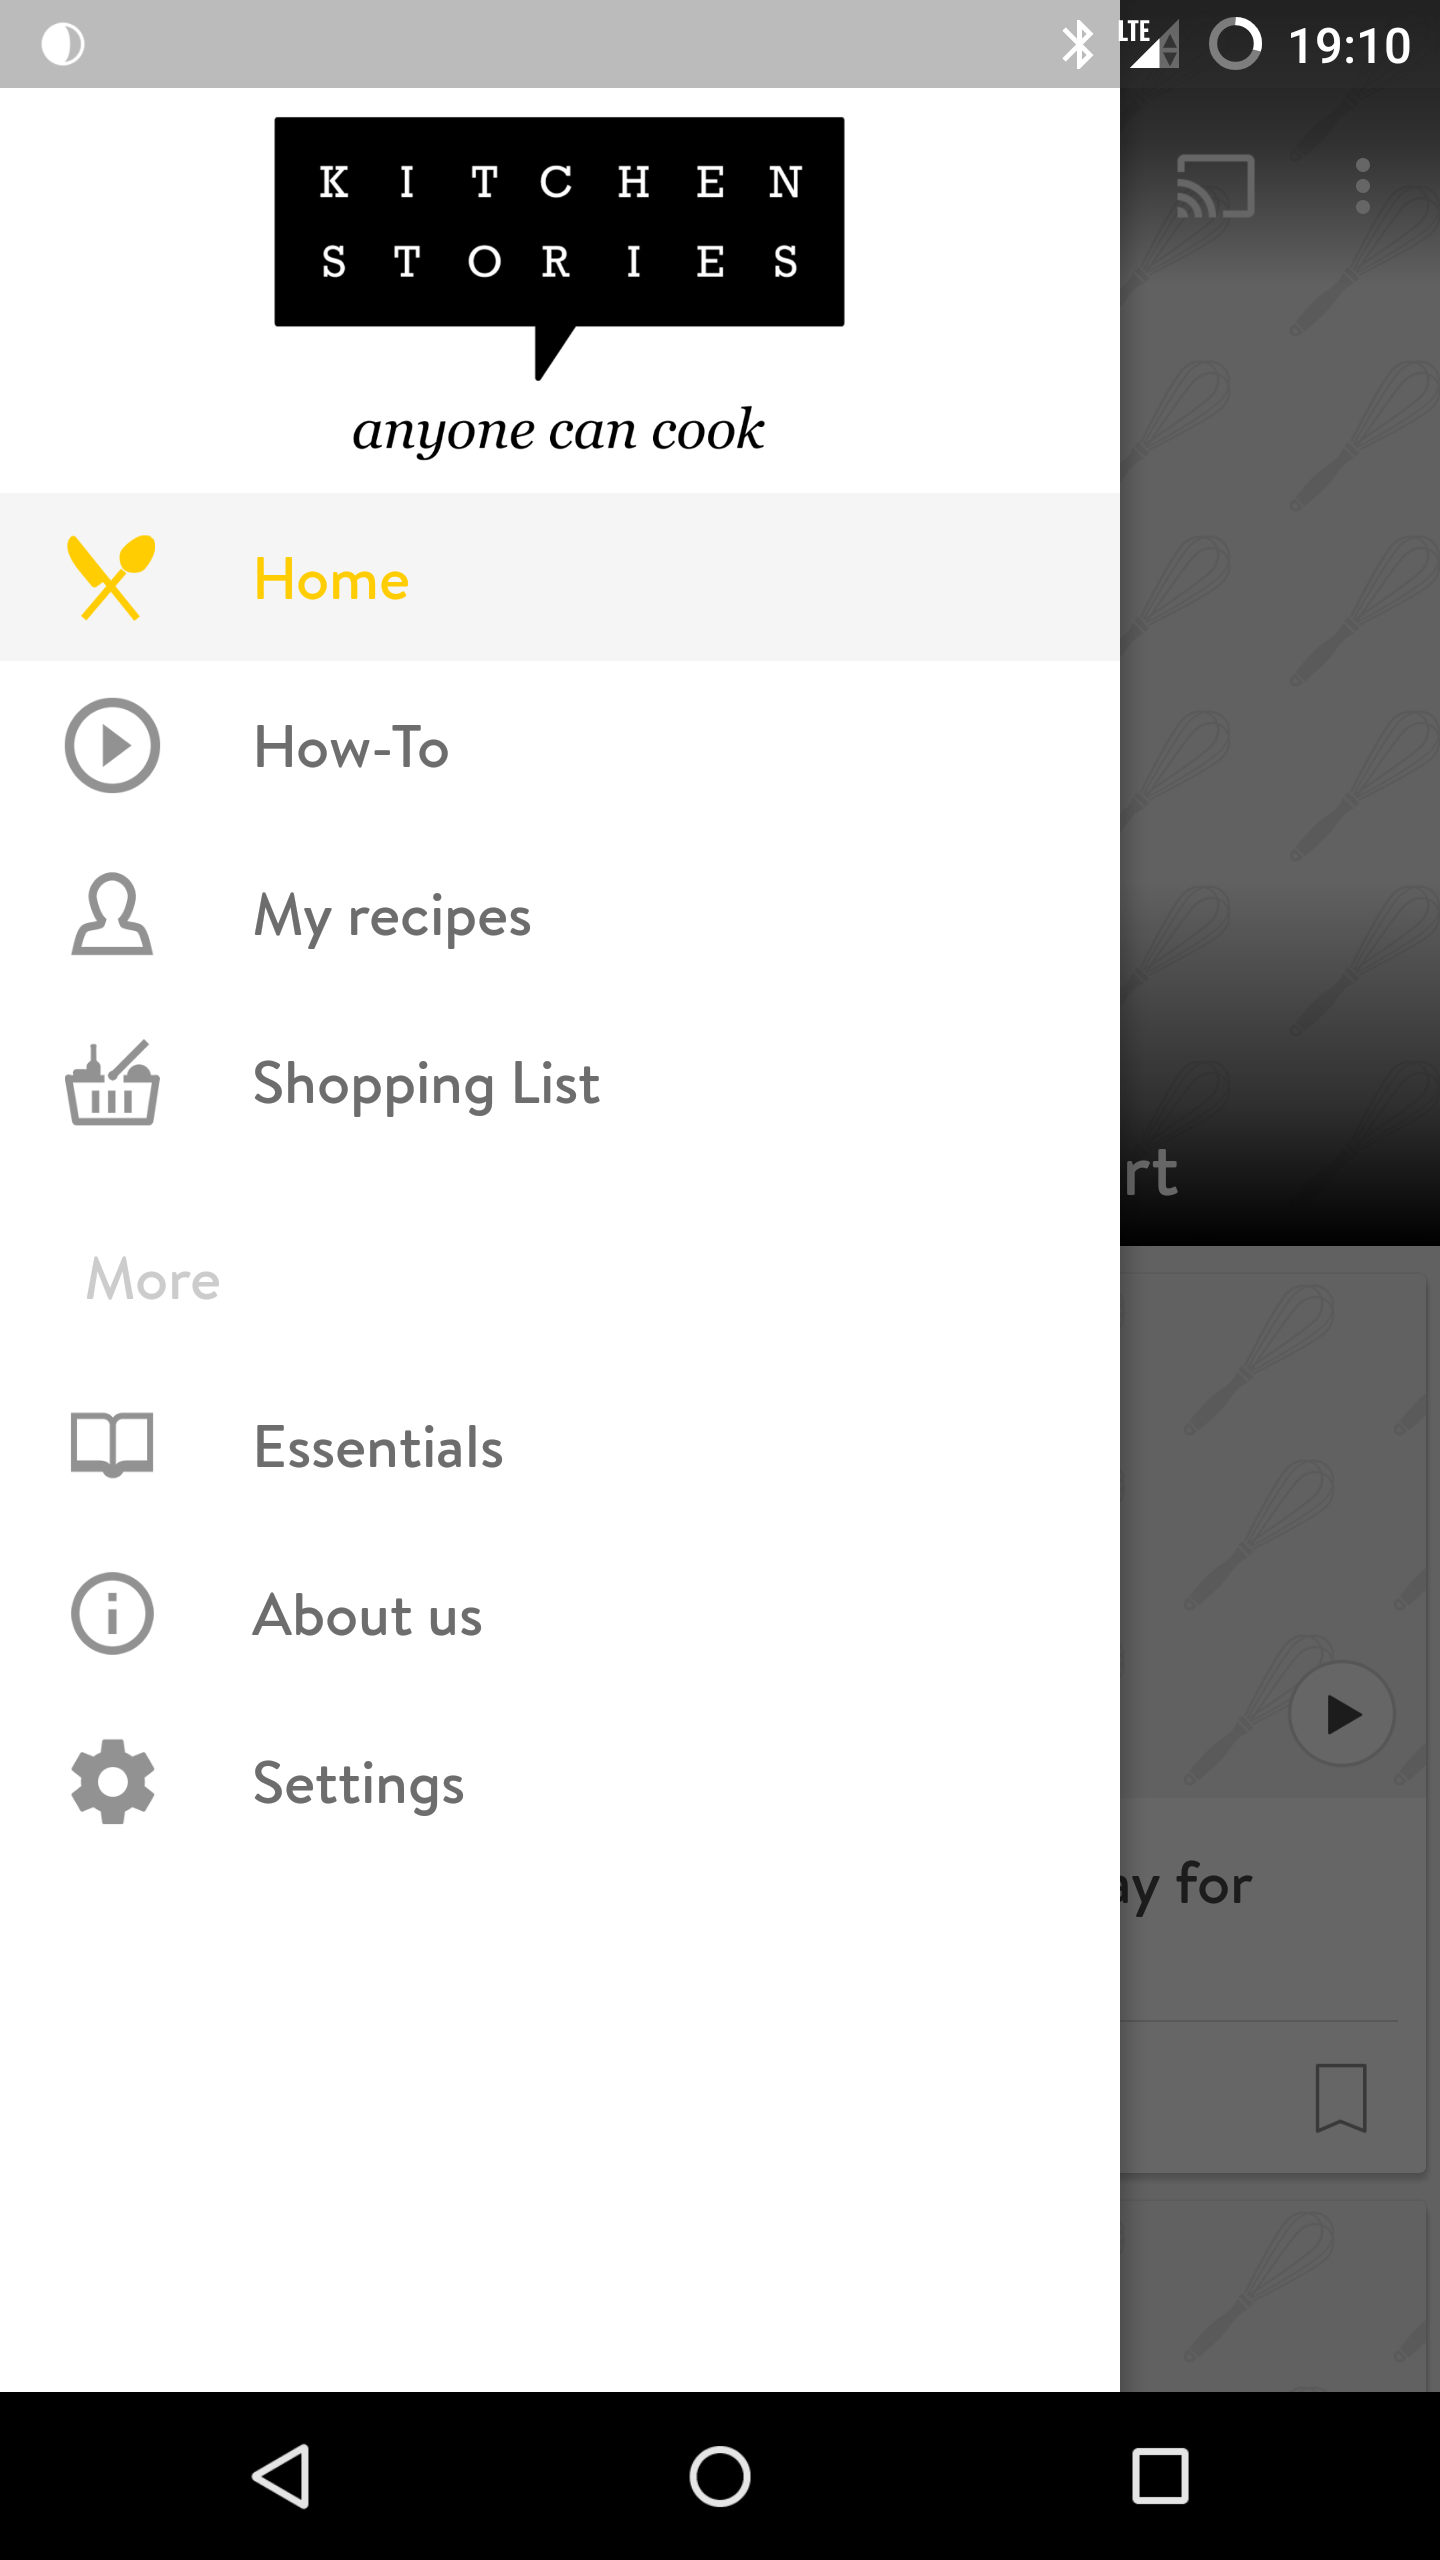
\includegraphics[scale=0.1]{figures/findings/open-nav-drawer-kitchenstories.png} }}%
	\caption{Example of an app with a closed navigation drawer (left) and an open navigation drawer (right).}
	\label{fig:nav_drawer}
\end{figure}
The navigation drawer is a hidden menu panel that can be revealed by tapping on the app icon menu (also known as the hamburger icon), which causes the panel to slide from left to right (figure~\ref{fig:nav_drawer}).
The navigation drawer has existed before the concepts of material design were introduced and was later added to the list of material design patterns with minor styling recommendation.
In order to create a navigation drawer, a developer needs to add a root element to the layout file with two children.
The root element must be a specific view called \textit{android.support.v4.widget.DrawerLayout}, which holds two children.
The first child can be any view group element to hold the content of the app.
The second child is a view that contains the content of the navigation drawer, which can be populated statically or dynamically with the drawer's list of items (e.g., \textit{ ListView} or \textit{android.support.design.widget.NavigationView}).
To find apps with a navigation drawer, I use the following Sieveable search queries:

\inputminted
[
framesep=2mm,
baselinestretch=1.2,
bgcolor=MyLightGrayColor,
fontsize=\footnotesize
]
{xml}{figures/source-code/navdrawer.txt}

\noindent These two search queries returned 20,165 unique apps in total.
To find the adoption rate of this design pattern over the years, I remove the duplicate apps from the results, keep the first version in which the adoption is observed, and group the remaining results by year.
Below, figure~\ref{fig:navdrawer_years} shows the adoption rate of the navigation drawer over the years from 2013 to 2016.
We can see an increase over the years but at a relatively slow rate (6.95\% is the average annual adoption increase).
\begin{figure}[h]
	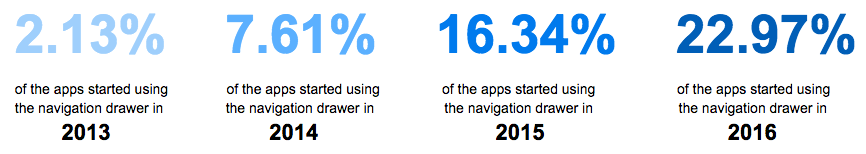
\includegraphics[scale=0.55]{figures/findings/navdrawer_over_years.png}
	\caption{The adoption rate of the Navigation Drawer over the years.}
	\label{fig:navdrawer_years}
\end{figure}
We can group the results by the release date quarterly and download count to see the trends in adopting this design pattern among most and less downloaded apps.
To better approximate the popularity of Android apps, I group the apps by download count into three main groups: a) most downloaded apps for apps with one million or more download times, b) middle downloaded apps for apps with 100,000 and fewer than 1,000,000 download counts, and c) least download apps for apps with fewer than 100,000 download counts.
Figure~\ref{fig:navdrawer_quarter_download} shows that the adoption rate of the navigation drawer is more prevalent in apps with the most download count than others with the exception of the first two quarters of 2015.
The analysis shows how the adoption of this design is changing after multiple major platform events.
We can see that this design is more adopted in top downloaded apps. 
It is also noticeable that it experienced a period of low popularity at some points in time but later gained a resurgence of interest after the release of an official library.

Analyzing apps over time enabled us to capture a correlation between design changes and major platform events.
UI design patterns may become more or less popular over time, but they may react positively to a related platform event.
This phenomena would have been missed had we considered a single version of the app.
Our finding suggests that the release of an official library (the design support library in this case) caused the adoption rate of the navigation drawer for apps that are less popular to soar.
We observed that apps with less download counts maintained an adoption rate below 10\% before the release of the official library, and that adoption doubled to over 20\% after the release of the library.
This event allowed developers of the less popular apps to close the gap and move forward to become close to top apps in design adoption.
\begin{figure}[H]
	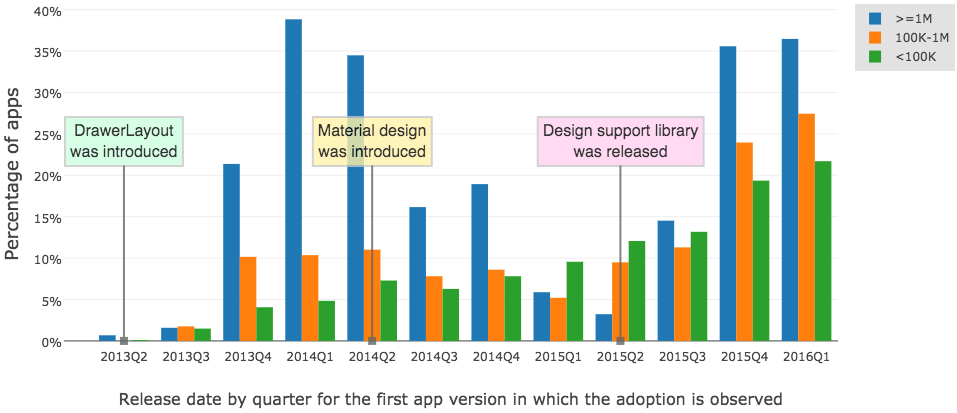
\includegraphics[scale=0.5]{figures/findings/navdrawer_by_quarter_grouped_by_downloads.png}
	\caption{The percentage of apps that started adopting the navigation drawer grouped by three download count groups: most, middle, and least downloaded apps. The x axis shows the calendar quarter of the release date in which the adoption is observed, and the y axis shows the percentage of apps that adopted it. The percentage value is computed by dividing the number of adopted apps in each quarter over the total of apps released in each quarter. The time of major platform events is also marked in the chart.}
	\label{fig:navdrawer_quarter_download}
\end{figure}

\section{Accessibility Mining Analysis}
The users of mobile devices are diverse with different physical capabilities including people with disabilities.
Some users may not be able to see the app, distinguish between its colors, touch the screen, hear a sound from the app, or speak back to the app.
Apps that are inaccessible to users with disabilities may exclude them from using important services and social activities.
Android features a set of accessibility APIs that help developers build accessible apps for users who have special needs.
Many research and development efforts are invested to address various accessibility issues and enhance existing system wide accessibility services.
Platform owners provide accessibility services, APIs, and guidelines to help developers improve the accessibility of their apps and increase their audiences.
Advancement in accessibility tools have wide range of benefits and applications to all users including users with no special needs.
For instance, some of the technologies that we use on daily basis started as an accessibility tools and evolved to benefit all users (e.g., speech recognition and word completion).
Even a user with no disability may experience accessibility restrictions in certain environments, i.e., when someone is not able to touch the device while driving, or distinguish between colors in a sunny environment.
Therefore, an app that is more accessible can benefit all users.
With all of these efforts in mind, I investigate the following question: are developers getting better in improving the accessibility of their apps?
In this section, I demonstrate how Sieveable can be used to answer this question and quantify the prevalence of accessibility violations over time.

\subsection{Accessibility Violation: Labeling Visual UI controls}
Modern mobile platform features accessibility guidelines that serve as a living document that is always updated with changes to the platform.
In android, the accessibility guidelines \cite{android_accessibility_guidelines} provide developers with a checklist of accessibility requirements \cite{android_accessibility_checklist} to help developers build more accessible applications.
The first item of this list is labeling visual user interface controls that do not have visible text.
This is a common accessibility violation in UI elements such as ImageButton and ImageView.
In many applications, UI controls use visual images to indicate the usage (e.g., a camera icon on an ImageButton to take a picture).
A UI control with no description text (also known as alternate text) is simply inaccessible to users with visual impairments.
It is worth noting that not all ImageView elements should be labeled since some are used for aesthetic purposes or visual spacing.
It is particularly important to label all ImageButton elements since they meant to represent an action in the app.
Thus, analyzing apps for the presence of labels in ImageButton elements tend to produce more accurate results than other UI elements.

One can use Sieveable to investigate the extent of this bug and whether developers pay attention to it over the years.
For instance, below are the search queries I use in this analysis.

\inputminted
[
framesep=2mm,
baselinestretch=1.2,
bgcolor=MyLightGrayColor,
fontsize=\footnotesize
]
{xml}{figures/source-code/image-btn-content-description.txt}

\noindent The first query is for finding apps that have an image button, while the last two queries are for finding apps that added a text label to an image button statically in layout files or dynamically in source code.
We can analyze the results of these search queries and compute the ratio of labeled image buttons in each app.
Figure~\ref{fig:img_btn_coverage_by_years} shows the average of accessible image button elements with text labels in all apps released from 2010 to 2016.
We observe around 5\% increase of accessible image buttons from 2012 to 2014 but that growth rate dropped to about 1\% in 2015 and 2016.

\begin{figure}[H]
	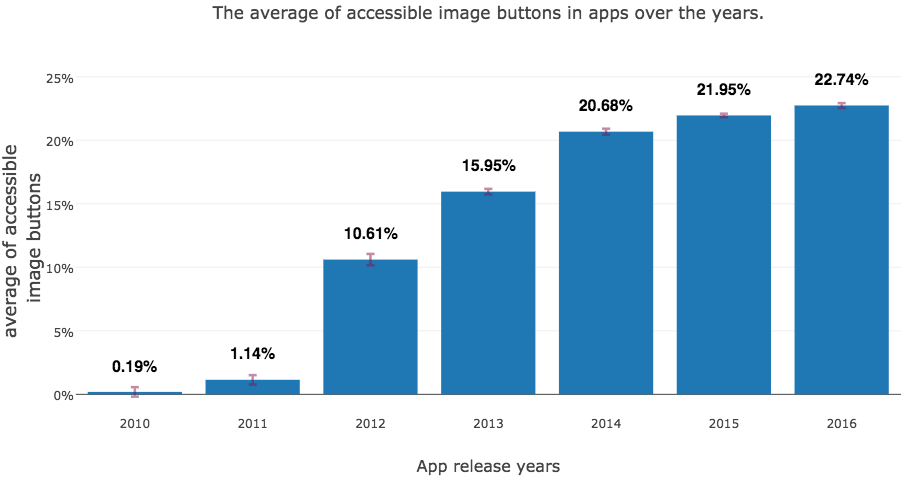
\includegraphics[scale=0.52]{./figures/findings/accessibility_accessible_image_btns_over_years.png}
	\caption{The percentage of accessible image buttons in apps over the release years. The error bars represent the standard deviations, which show the variation among average values.}
	\label{fig:img_btn_coverage_by_years}
\end{figure}
\begin{figure}[H]
	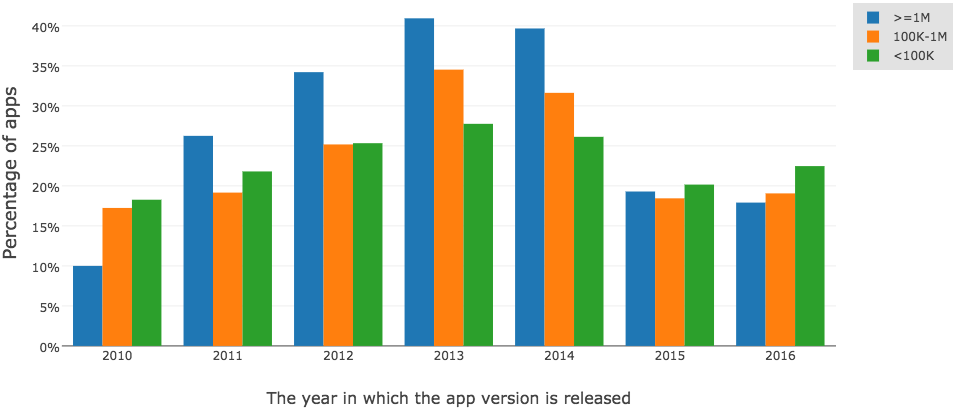
\includegraphics[scale=0.55]{figures/findings/accessibility_inaccessible_image_btns_by_year_and_download.png}
	\caption{The percentage of apps that have no accessible ImageButton elements grouped by download count and release year.}
	\label{fig:img_btn_no_coverage_by_years}
\end{figure}
We can also sample the apps with no accessible image buttons (i.e. an app that has no label for all of its image buttons) and group them by download count.
I used the results of the third search query to provide a more accurate estimate of apps that do not label image buttons statically or dynamically,
Figure~\ref{fig:img_btn_no_coverage_by_years} shows the percentage of apps in three download count groups (top, middle, and bottom) that had no text labels in all the image buttons they used.
This result shows that this accessibility bug is common across all apps of different download times. 
It was even more common in the top downloaded apps in from 2011 to 2014.
However, it dropped in the following two years to become relatively common in all three download count groups.

The results of this analysis show a mixed view of accessibility improvements in Android apps over the years.
While we have seen a small yet noticeable improvement in the years before 2015 but that growth rate dropped later in the following years.
These findings prove that accessibility is still a problem for many of the most downloaded and popular apps.
In addition, the results also highlight the severity of this accessibility problem across all apps with all popularity levels.
The results presented here highlight the potential of using Sieveable in future work to estimate the accessibility of mobile apps over time and address accessibility problems.

\section{Security Mining Analysis}
